\section{Supervised Learning}%
\label{sec:supervised}

\begin{frame}{Machine Learning Workflow}
  \begin{figure}[!htbp]
    \centering
    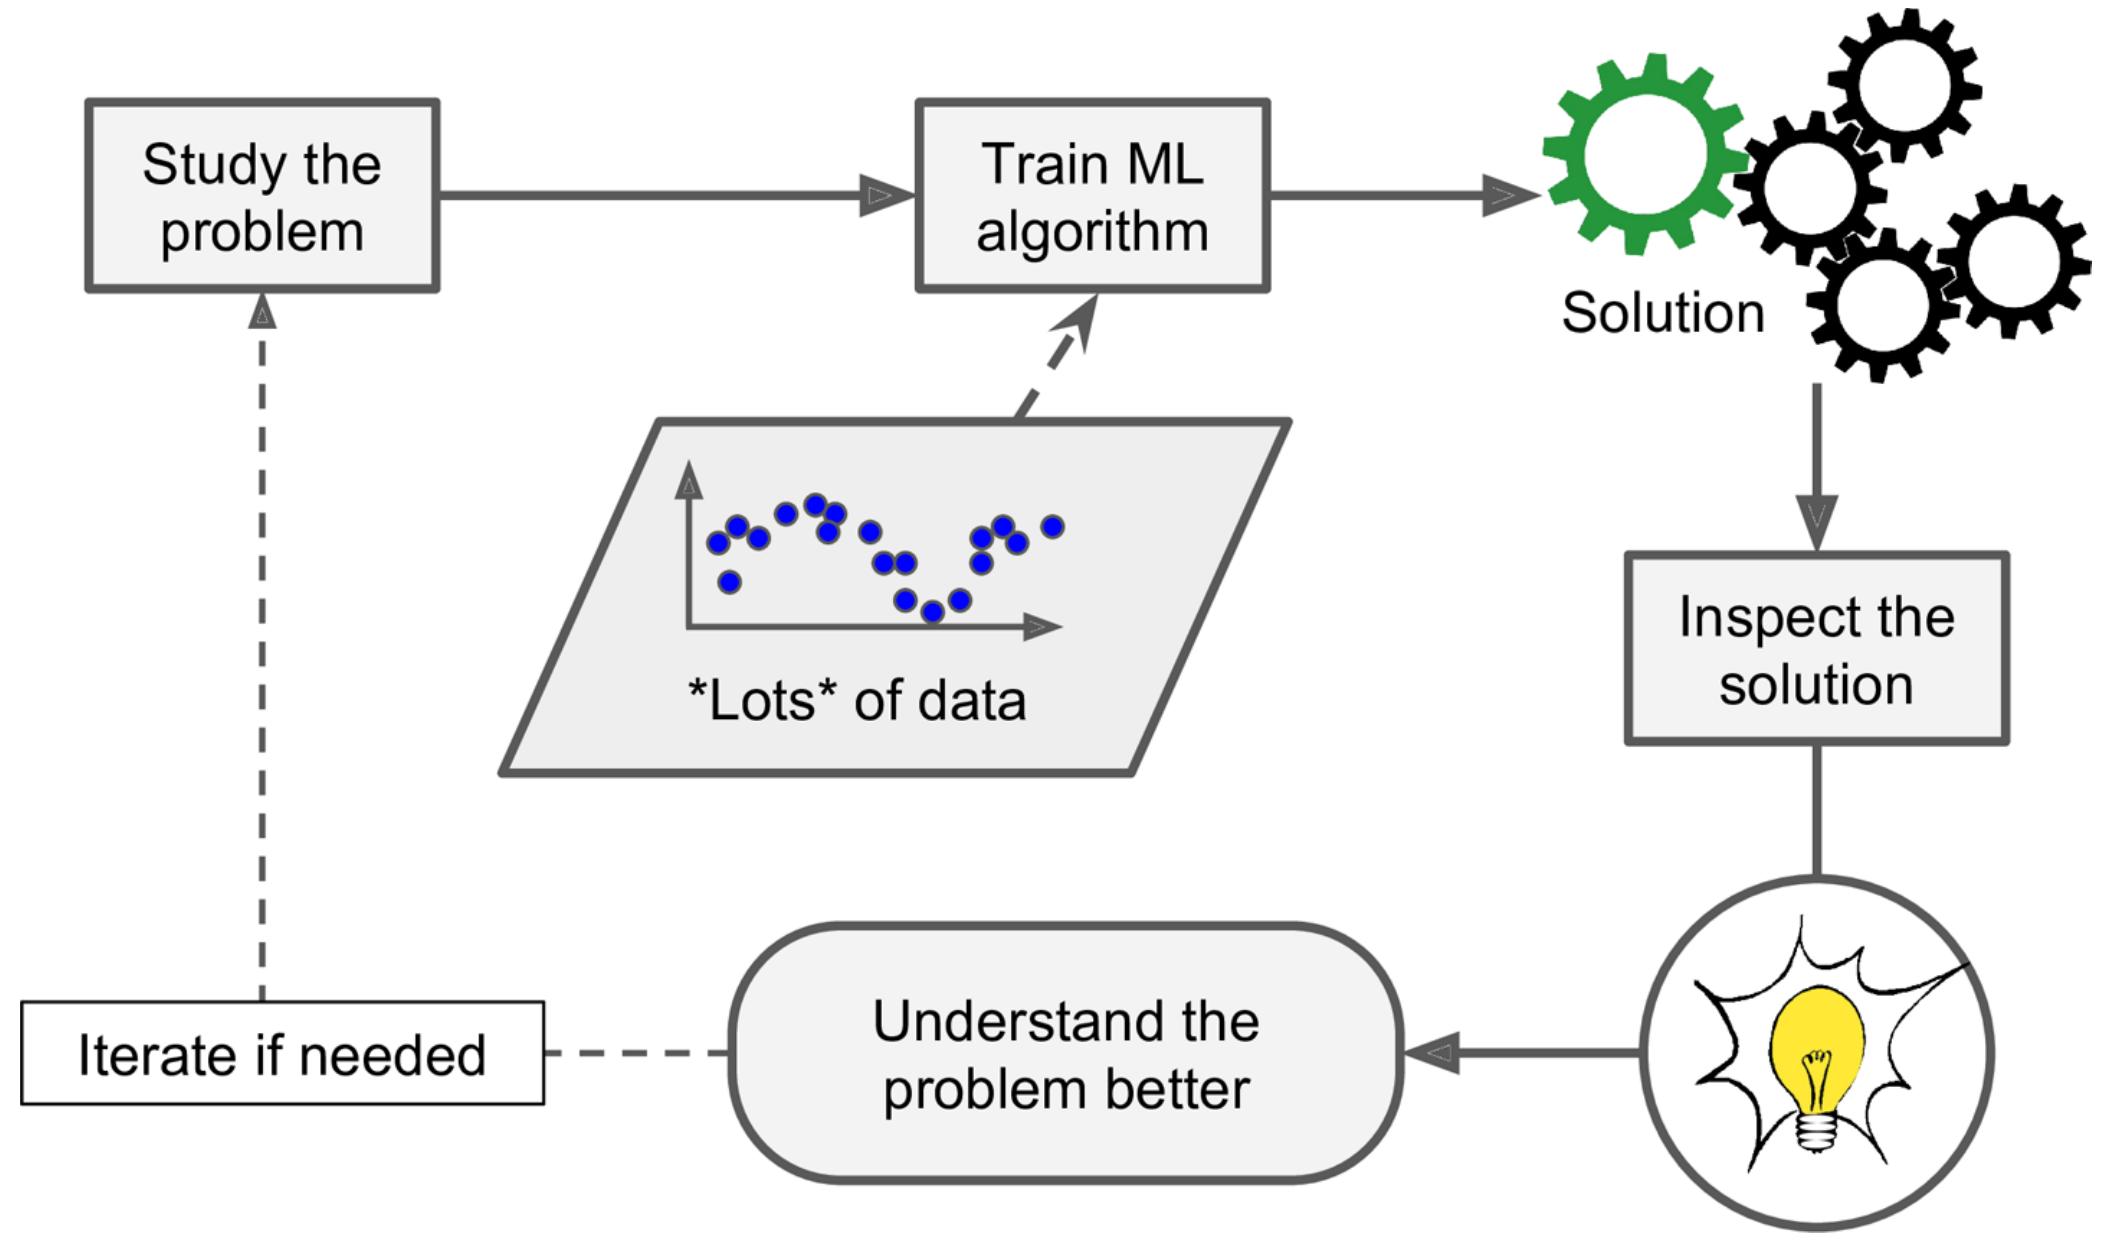
\includegraphics[width=10cm]{ml_workflow}
    \caption{Machine Learning Workflow \parencite{geron2019hands}}%
    \label{fig:workflow}
  \end{figure}
\end{frame}

\begin{frame}{Supervised Learning}
  \begin{figure}[!htbp]
    \centering
    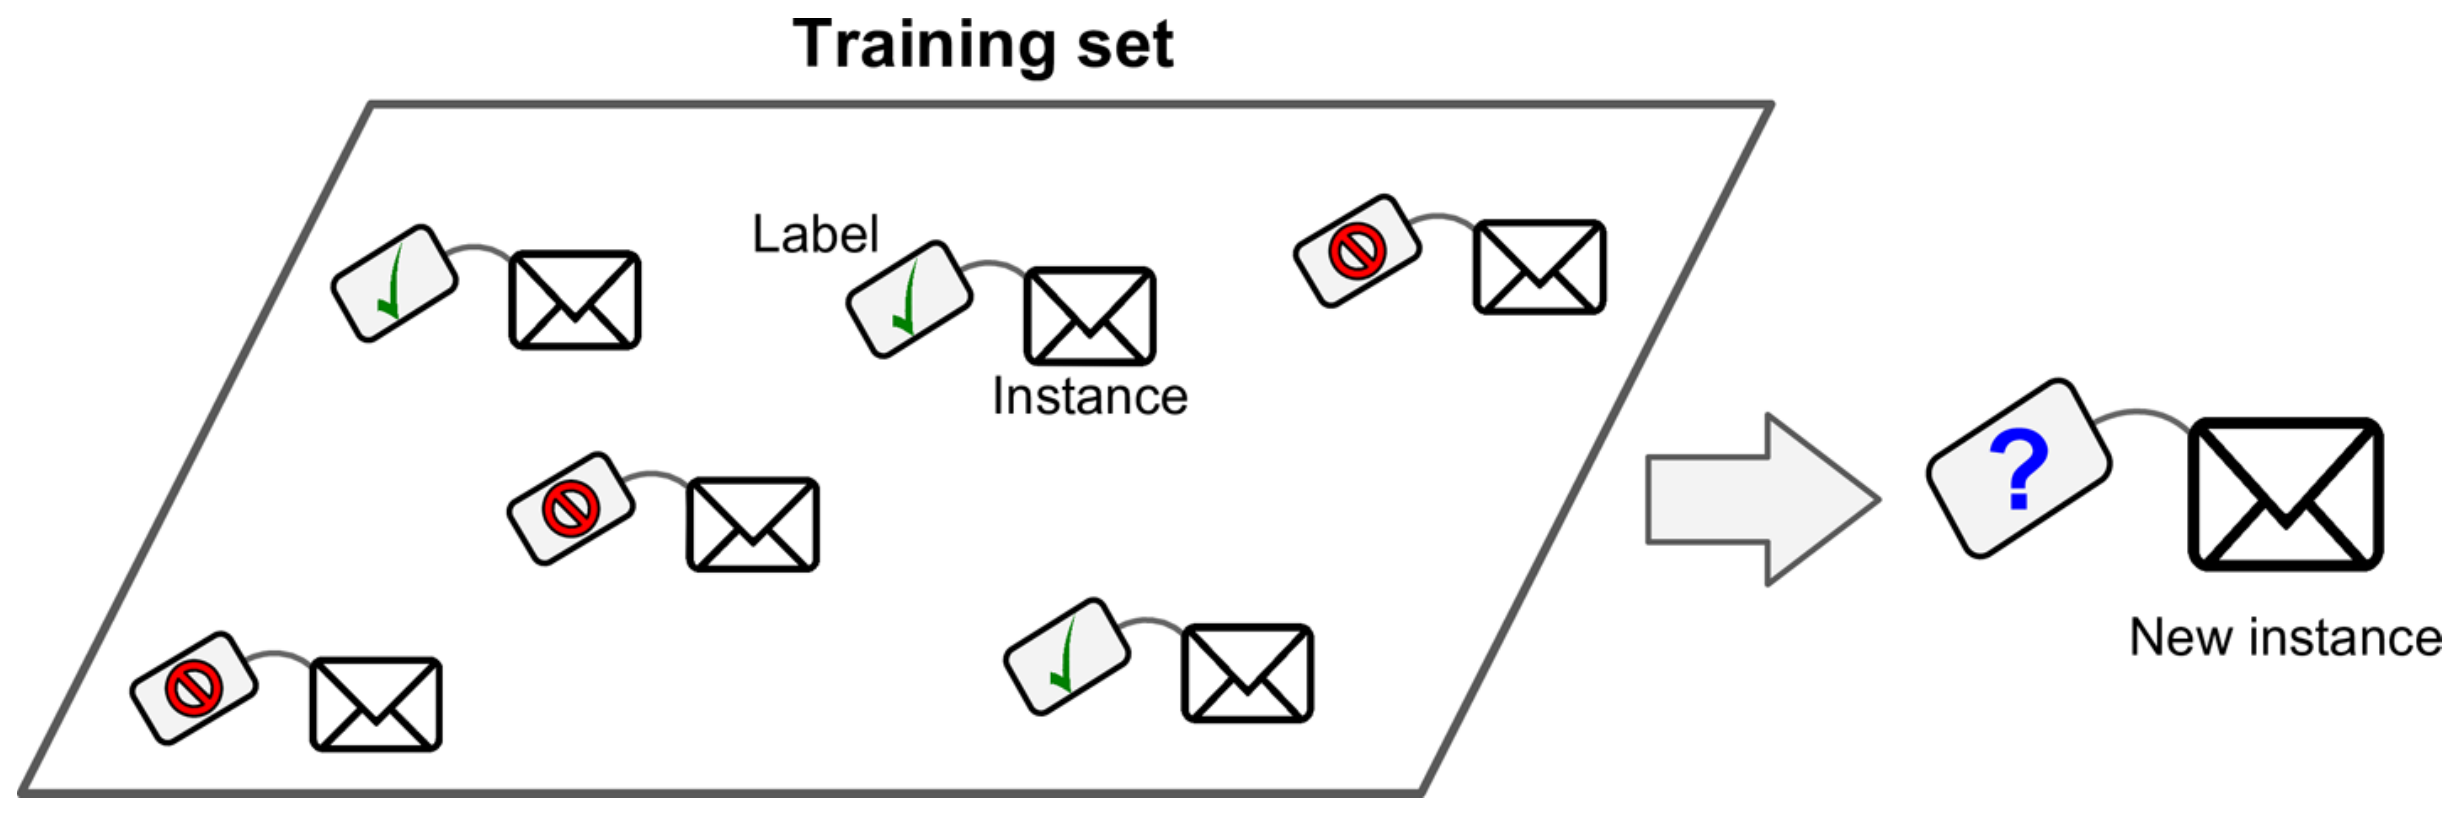
\includegraphics[width=8cm]{data}
    \caption{Struktur der Daten bei Supervised Learning \parencite{geron2019hands}}%
    \label{fig:data}
  \end{figure}

  \only<2->{
    \small
    \begin{block}{Definition Supervised Learning}
      \enquote{In supervised learning, the dataset is the collection of labeled examples
      \({\{(\mathbf{x}_i, y_i)\}}_{i=1}^N\). Each element \(\mathbf{x}_i\) among
      \(N\) is called a feature vector. A feature vector is a vector in which each
      dimension \(j = 1, \ldots , D\) contains a value that describes the example
      somehow [\ldots]. The goal of a supervised learning algorithm is to use the
      dataset to produce a model, that takes a feature vector \(\mathbf{x}\) as
      input and outputs information that allow deducing the label \(\hat{y}\) for
      this feature vector.} \parencite{burkov2019hundred}
    \end{block}
  }
\end{frame}

\begin{frame}{Beispiel: Datensatz für Supervised Learning}
  \begin{minipage}{.6\textwidth}
    \centering
    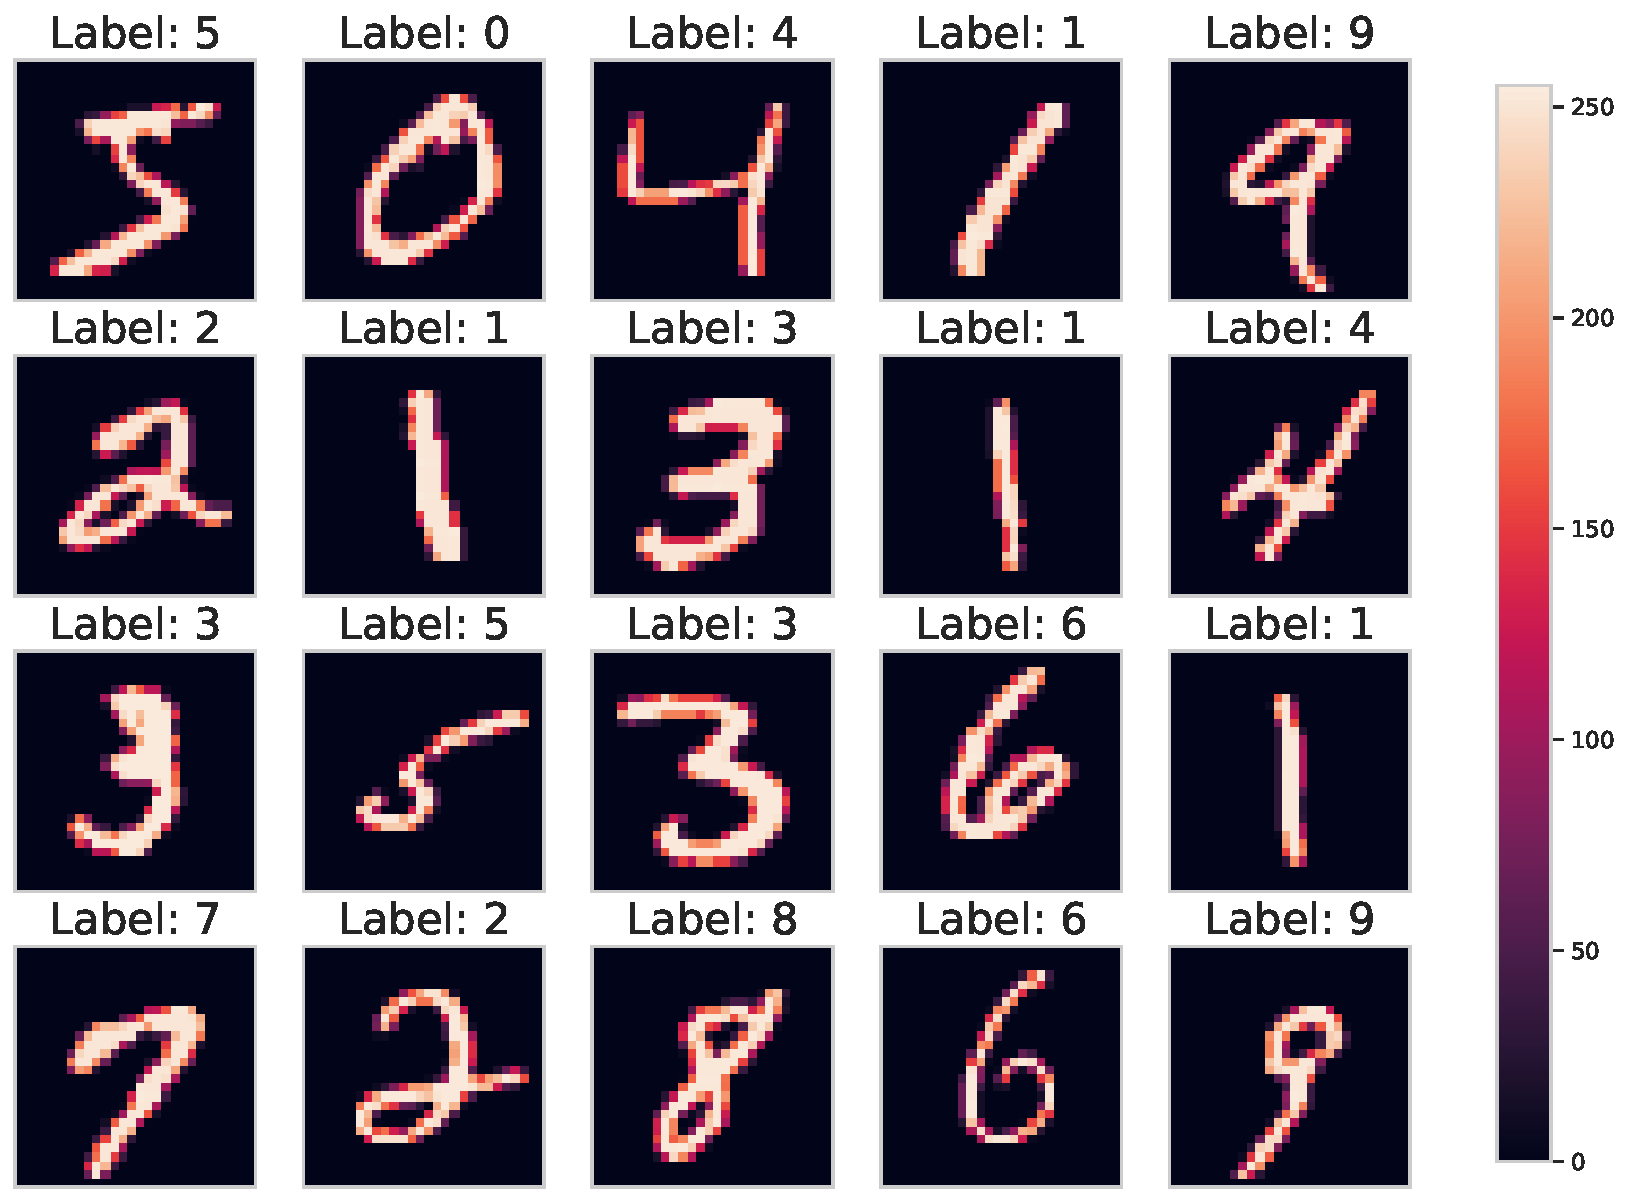
\includegraphics[width=\textwidth]{mnist}
  \end{minipage}\hfill%
  \begin{minipage}{.4\textwidth}
    \begin{itemize}
    \item Insgesamt 70000 Bilder
    \item Bildgröße: 28 \(\times\) 28 Pixel
    \item Abgebildet: Handgeschriebene Ziffern von 0 bis 9
    \item Quelle: Yann LeCun et al \parencite{lecun1998gradient}
    \end{itemize}
  \end{minipage}
\end{frame}

\begin{frame}{Beispiel: Datensatz für Supervised Learning}
  \begin{minipage}{.6\textwidth}
    \centering 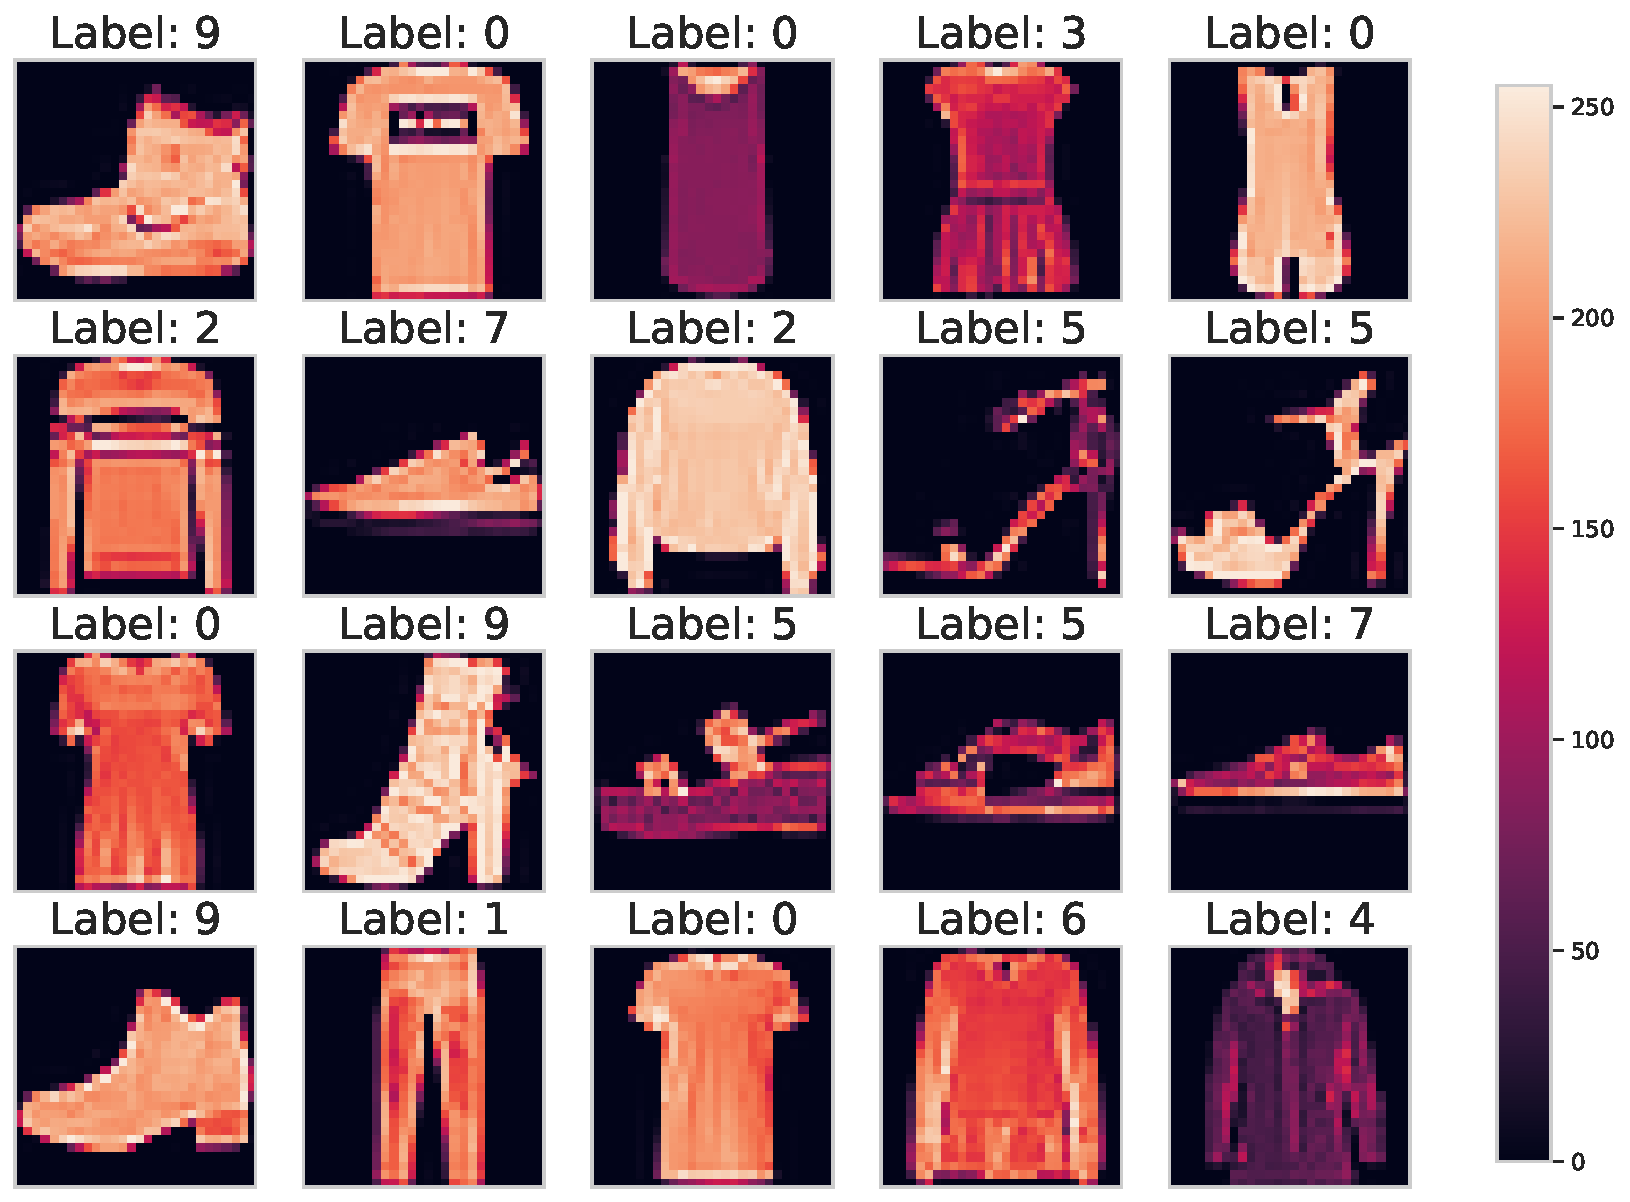
\includegraphics[width=\textwidth]{fashion_mnist}
  \end{minipage}\hfill%
  \begin{minipage}{.4\textwidth}
    \begin{itemize}
    \item Insgesamt 70000 Bilder
    \item Bildgröße: 28 \(\times\) 28 Pixel
    \item Abgebildet: Kleidungsstücke 
    \item Quelle: Zalando Research \parencite{xiao2017fashion}
    \end{itemize}

    \vspace{.5cm}

    \tiny

    \centering
    \begin{tabular}{ll}
      \toprule
      \textbf{Label} & 	\textbf{Description}\\
      \midrule
      0 & 	T-shirt/top\\
      1 & 	Trouser\\
      2 & 	Pullover\\
      3 & 	Dress\\
      4 & 	Coat\\
      5 & 	Sandal\\
      6 & 	Shirt\\
      7 & 	Sneaker\\
      8 & 	Bag\\
      9 & 	Ankle boot\\
      \bottomrule
    \end{tabular}

  \end{minipage}

\end{frame}

%%% Local Variables:
%%% mode: latex
%%% TeX-master: "../präsentation"
%%% End:
